\documentclass[a4,12pt]{article}
\usepackage{colortbl}
\usepackage{pgfplots}
\usepackage[margin=2cm]{geometry}
\pgfplotsset{compat=newest}
\begin{document}
\begin{table}
\footnotesize
\sffamily
\begin{center}
\begin{tabular}{cccccccccc}
Mean-Accuracy & \shortstack{MMM4TSC \\ 0.7940} & \shortstack{LITETime \\ 0.7929} & \shortstack{InceptionTime \\ 0.7924} & \shortstack{Inception \\ 0.7807} & \shortstack{ROCKET \\ 0.7733} & \shortstack{LITE \\ 0.7694} & \shortstack{ResNet \\ 0.7491} & \shortstack{FCN \\ 0.7276} \\[1ex]
\shortstack{MMM4TSC \\ 0.7940} & \cellcolor[rgb]{0.8674,0.8644,0.8626}\shortstack{\rule{0em}{3ex} Mean-Difference \\ r$>$c / r=c / r$<$c \\ Wilcoxon p-value} & \cellcolor[rgb]{0.8715,0.8623,0.857}\shortstack{\rule{0em}{3ex} 0.0011 \\ 16 / 0 / 19 \\ 0.7524} & \cellcolor[rgb]{0.8756,0.8602,0.8514}\shortstack{\rule{0em}{3ex} 0.0016 \\ 16 / 0 / 19 \\ 0.6330} & \cellcolor[rgb]{0.9383,0.8089,0.7412}\shortstack{\rule{0em}{3ex} 0.0133 \\ 19 / 0 / 16 \\ 0.2071} & \cellcolor[rgb]{0.9606,0.7625,0.668}\shortstack{\rule{0em}{3ex} 0.0207 \\ 20 / 0 / 15 \\ 0.2318} & \bfseries \cellcolor[rgb]{0.967,0.7357,0.6309}\shortstack{\rule{0em}{3ex} 0.0246 \\ 21 / 0 / 14 \\ 0.0371} & \bfseries \cellcolor[rgb]{0.9417,0.5464,0.4297}\shortstack{\rule{0em}{3ex} 0.0449 \\ 20 / 1 / 14 \\ 0.0078} & \bfseries \cellcolor[rgb]{0.8204,0.2868,0.2452}\shortstack{\rule{0em}{3ex} 0.0664 \\ 26 / 0 / 9 \\  $\leq$ 1e-04} \\[1ex]
\shortstack{LITETime \\ 0.7929} & \cellcolor[rgb]{0.8594,0.8644,0.8721}\shortstack{\rule{0em}{3ex} -0.0011 \\ 19 / 0 / 16 \\ 0.7524} & \cellcolor[rgb]{0.8674,0.8644,0.8626}\shortstack{\rule{0em}{3ex} -} & \cellcolor[rgb]{0.8674,0.8644,0.8626}\shortstack{\rule{0em}{3ex} 0.0004 \\ 13 / 3 / 19 \\ 0.8763} & \bfseries \cellcolor[rgb]{0.9332,0.8156,0.7532}\shortstack{\rule{0em}{3ex} 0.0122 \\ 25 / 0 / 10 \\ 0.0091} & \cellcolor[rgb]{0.9582,0.7712,0.6803}\shortstack{\rule{0em}{3ex} 0.0196 \\ 23 / 0 / 12 \\ 0.1843} & \bfseries \cellcolor[rgb]{0.9648,0.7446,0.6432}\shortstack{\rule{0em}{3ex} 0.0235 \\ 34 / 0 / 1 \\  $\leq$ 1e-04} & \bfseries \cellcolor[rgb]{0.9459,0.5596,0.4415}\shortstack{\rule{0em}{3ex} 0.0438 \\ 28 / 1 / 6 \\  $\leq$ 1e-04} & \bfseries \cellcolor[rgb]{0.8302,0.3047,0.2549}\shortstack{\rule{0em}{3ex} 0.0653 \\ 33 / 0 / 2 \\  $\leq$ 1e-04} \\[1ex]
\shortstack{InceptionTime \\ 0.7924} & \cellcolor[rgb]{0.8554,0.8638,0.8766}\shortstack{\rule{0em}{3ex} -0.0016 \\ 19 / 0 / 16 \\ 0.6330} & \cellcolor[rgb]{0.8634,0.8651,0.8676}\shortstack{\rule{0em}{3ex} -0.0004 \\ 19 / 3 / 13 \\ 0.8763} & \cellcolor[rgb]{0.8674,0.8644,0.8626}\shortstack{\rule{0em}{3ex} -} & \bfseries \cellcolor[rgb]{0.9307,0.8189,0.7591}\shortstack{\rule{0em}{3ex} 0.0117 \\ 33 / 1 / 1 \\  $\leq$ 1e-04} & \cellcolor[rgb]{0.9564,0.7751,0.6864}\shortstack{\rule{0em}{3ex} 0.0192 \\ 21 / 1 / 13 \\ 0.1714} & \bfseries \cellcolor[rgb]{0.9648,0.7446,0.6432}\shortstack{\rule{0em}{3ex} 0.0230 \\ 25 / 0 / 10 \\ 0.0034} & \bfseries \cellcolor[rgb]{0.9477,0.566,0.4475}\shortstack{\rule{0em}{3ex} 0.0434 \\ 29 / 1 / 5 \\  $\leq$ 1e-04} & \bfseries \cellcolor[rgb]{0.8302,0.3047,0.2549}\shortstack{\rule{0em}{3ex} 0.0648 \\ 32 / 0 / 3 \\  $\leq$ 1e-04} \\[1ex]
\shortstack{Inception \\ 0.7807} & \cellcolor[rgb]{0.7727,0.839,0.9493}\shortstack{\rule{0em}{3ex} -0.0133 \\ 16 / 0 / 19 \\ 0.2071} & \bfseries \cellcolor[rgb]{0.782,0.8429,0.943}\shortstack{\rule{0em}{3ex} -0.0122 \\ 10 / 0 / 25 \\ 0.0091} & \bfseries \cellcolor[rgb]{0.7867,0.8448,0.9398}\shortstack{\rule{0em}{3ex} -0.0117 \\ 1 / 1 / 33 \\  $\leq$ 1e-04} & \cellcolor[rgb]{0.8674,0.8644,0.8626}\shortstack{\rule{0em}{3ex} -} & \cellcolor[rgb]{0.9095,0.8394,0.8003}\shortstack{\rule{0em}{3ex} 0.0074 \\ 18 / 0 / 17 \\ 0.7647} & \cellcolor[rgb]{0.9307,0.8189,0.7591}\shortstack{\rule{0em}{3ex} 0.0113 \\ 19 / 1 / 15 \\ 0.7556} & \bfseries \cellcolor[rgb]{0.9689,0.6795,0.5628}\shortstack{\rule{0em}{3ex} 0.0316 \\ 24 / 0 / 11 \\ 0.0040} & \bfseries \cellcolor[rgb]{0.9058,0.4552,0.3553}\shortstack{\rule{0em}{3ex} 0.0531 \\ 28 / 0 / 7 \\ 0.0001} \\[1ex]
\shortstack{ROCKET \\ 0.7733} & \cellcolor[rgb]{0.7139,0.8089,0.9794}\shortstack{\rule{0em}{3ex} -0.0207 \\ 15 / 0 / 20 \\ 0.2318} & \cellcolor[rgb]{0.724,0.8149,0.9757}\shortstack{\rule{0em}{3ex} -0.0196 \\ 12 / 0 / 23 \\ 0.1843} & \cellcolor[rgb]{0.729,0.8175,0.9732}\shortstack{\rule{0em}{3ex} -0.0192 \\ 13 / 1 / 21 \\ 0.1714} & \cellcolor[rgb]{0.8181,0.8556,0.9146}\shortstack{\rule{0em}{3ex} -0.0074 \\ 17 / 0 / 18 \\ 0.7647} & \cellcolor[rgb]{0.8674,0.8644,0.8626}\shortstack{\rule{0em}{3ex} -} & \cellcolor[rgb]{0.8918,0.852,0.8291}\shortstack{\rule{0em}{3ex} 0.0039 \\ 18 / 0 / 17 \\ 0.5329} & \cellcolor[rgb]{0.9659,0.7401,0.6371}\shortstack{\rule{0em}{3ex} 0.0242 \\ 22 / 0 / 13 \\ 0.0557} & \bfseries \cellcolor[rgb]{0.9393,0.5396,0.4239}\shortstack{\rule{0em}{3ex} 0.0457 \\ 26 / 0 / 9 \\ 0.0013} \\[1ex]
\shortstack{LITE \\ 0.7694} & \bfseries \cellcolor[rgb]{0.6831,0.79,0.9898}\shortstack{\rule{0em}{3ex} -0.0246 \\ 14 / 0 / 21 \\ 0.0356} & \bfseries \cellcolor[rgb]{0.6933,0.7963,0.9863}\shortstack{\rule{0em}{3ex} -0.0235 \\ 1 / 0 / 34 \\  $\leq$ 1e-04} & \bfseries \cellcolor[rgb]{0.6933,0.7963,0.9863}\shortstack{\rule{0em}{3ex} -0.0230 \\ 10 / 0 / 25 \\ 0.0034} & \cellcolor[rgb]{0.7867,0.8448,0.9398}\shortstack{\rule{0em}{3ex} -0.0113 \\ 15 / 1 / 19 \\ 0.7556} & \cellcolor[rgb]{0.8394,0.8612,0.8945}\shortstack{\rule{0em}{3ex} -0.0039 \\ 17 / 0 / 18 \\ 0.5223} & \cellcolor[rgb]{0.8674,0.8644,0.8626}\shortstack{\rule{0em}{3ex} -} & \cellcolor[rgb]{0.9595,0.767,0.6741}\shortstack{\rule{0em}{3ex} 0.0203 \\ 24 / 0 / 11 \\ 0.0649} & \bfseries \cellcolor[rgb]{0.9513,0.5788,0.4594}\shortstack{\rule{0em}{3ex} 0.0418 \\ 27 / 2 / 6 \\ 0.0001} \\[1ex]
\shortstack{ResNet \\ 0.7491} & \bfseries \cellcolor[rgb]{0.5054,0.644,0.9832}\shortstack{\rule{0em}{3ex} -0.0449 \\ 14 / 1 / 20 \\ 0.0078} & \bfseries \cellcolor[rgb]{0.5163,0.6545,0.9864}\shortstack{\rule{0em}{3ex} -0.0438 \\ 6 / 1 / 28 \\  $\leq$ 1e-04} & \bfseries \cellcolor[rgb]{0.5217,0.6596,0.9877}\shortstack{\rule{0em}{3ex} -0.0434 \\ 5 / 1 / 29 \\  $\leq$ 1e-04} & \bfseries \cellcolor[rgb]{0.6247,0.7483,0.9987}\shortstack{\rule{0em}{3ex} -0.0316 \\ 11 / 0 / 24 \\ 0.0040} & \cellcolor[rgb]{0.6882,0.7932,0.988}\shortstack{\rule{0em}{3ex} -0.0242 \\ 13 / 0 / 22 \\ 0.0557} & \cellcolor[rgb]{0.719,0.812,0.9777}\shortstack{\rule{0em}{3ex} -0.0203 \\ 11 / 0 / 24 \\ 0.0625} & \cellcolor[rgb]{0.8674,0.8644,0.8626}\shortstack{\rule{0em}{3ex} -} & \bfseries \cellcolor[rgb]{0.9616,0.758,0.6618}\shortstack{\rule{0em}{3ex} 0.0215 \\ 25 / 0 / 10 \\ 0.0032} \\[1ex]
\shortstack{FCN \\ 0.7276} & \bfseries \cellcolor[rgb]{0.3286,0.4397,0.8696}\shortstack{\rule{0em}{3ex} -0.0664 \\ 9 / 0 / 26 \\  $\leq$ 1e-04} & \bfseries \cellcolor[rgb]{0.3384,0.4528,0.8793}\shortstack{\rule{0em}{3ex} -0.0653 \\ 2 / 0 / 33 \\  $\leq$ 1e-04} & \bfseries \cellcolor[rgb]{0.3384,0.4528,0.8793}\shortstack{\rule{0em}{3ex} -0.0648 \\ 3 / 0 / 32 \\  $\leq$ 1e-04} & \bfseries \cellcolor[rgb]{0.4358,0.5707,0.9517}\shortstack{\rule{0em}{3ex} -0.0531 \\ 7 / 0 / 28 \\ 0.0001} & \bfseries \cellcolor[rgb]{0.5,0.6385,0.9811}\shortstack{\rule{0em}{3ex} -0.0457 \\ 9 / 0 / 26 \\ 0.0013} & \bfseries \cellcolor[rgb]{0.5326,0.6698,0.9904}\shortstack{\rule{0em}{3ex} -0.0418 \\ 6 / 2 / 27 \\ 0.0001} & \bfseries \cellcolor[rgb]{0.7087,0.8057,0.9811}\shortstack{\rule{0em}{3ex} -0.0215 \\ 10 / 0 / 25 \\ 0.0030} & \cellcolor[rgb]{0.8674,0.8644,0.8626}\shortstack{\rule{0em}{3ex} If in bold, then \\ p-value $<$ 0.05} \\[1ex]
\end{tabular}
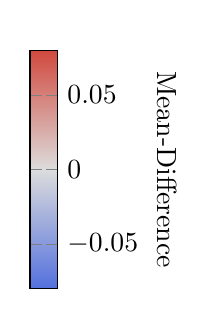
\begin{tikzpicture}[baseline=(current bounding box.center)]\begin{axis}[hide axis,scale only axis,width=1pt,colorbar right,colorbar style={height=0.25\linewidth,colormap={cm}{rgb255(1)=(83,112,221) rgb255(2)=(220,220,220) rgb255(3)=(209,73,62)},colorbar horizontal,point meta min=-0.08,point meta max=0.08,colorbar/width=1.0em,scaled y ticks=false,ylabel style={rotate=180},yticklabel style={/pgf/number format/fixed,/pgf/number format/precision=3},ylabel={Mean-Difference},}] \addplot[draw=none] {0};\end{axis}\end{tikzpicture}\end{center}
\caption{[...] \textbf{If in bold, then p-value $<$ 0.05} [...]}
\end{table}
\end{document}
